\documentclass[11pt]{beamer}
\usetheme{Frankfurt}
\usepackage[utf8]{inputenc}
\usepackage[german]{babel}
\usepackage{amsmath}
\usepackage{amsfonts}
\usepackage{amssymb}
\usepackage{graphicx}
\author{Valerie Wiedemann}
\title{Projektpräsentation}
%\setbeamercovered{transparent} 
%\setbeamertemplate{navigation symbols}{} 
%\logo{} 
%\institute{} 
\date{29. Oktober 2015} 
%\subject{} 
\begin{document}

\begin{frame}
\titlepage
\end{frame}

%\begin{frame}
%\tableofcontents
%\end{frame}

%Garagen zu
\begin{frame}{Problem}
\begin{figure}[h]
\makebox[\textwidth]{
 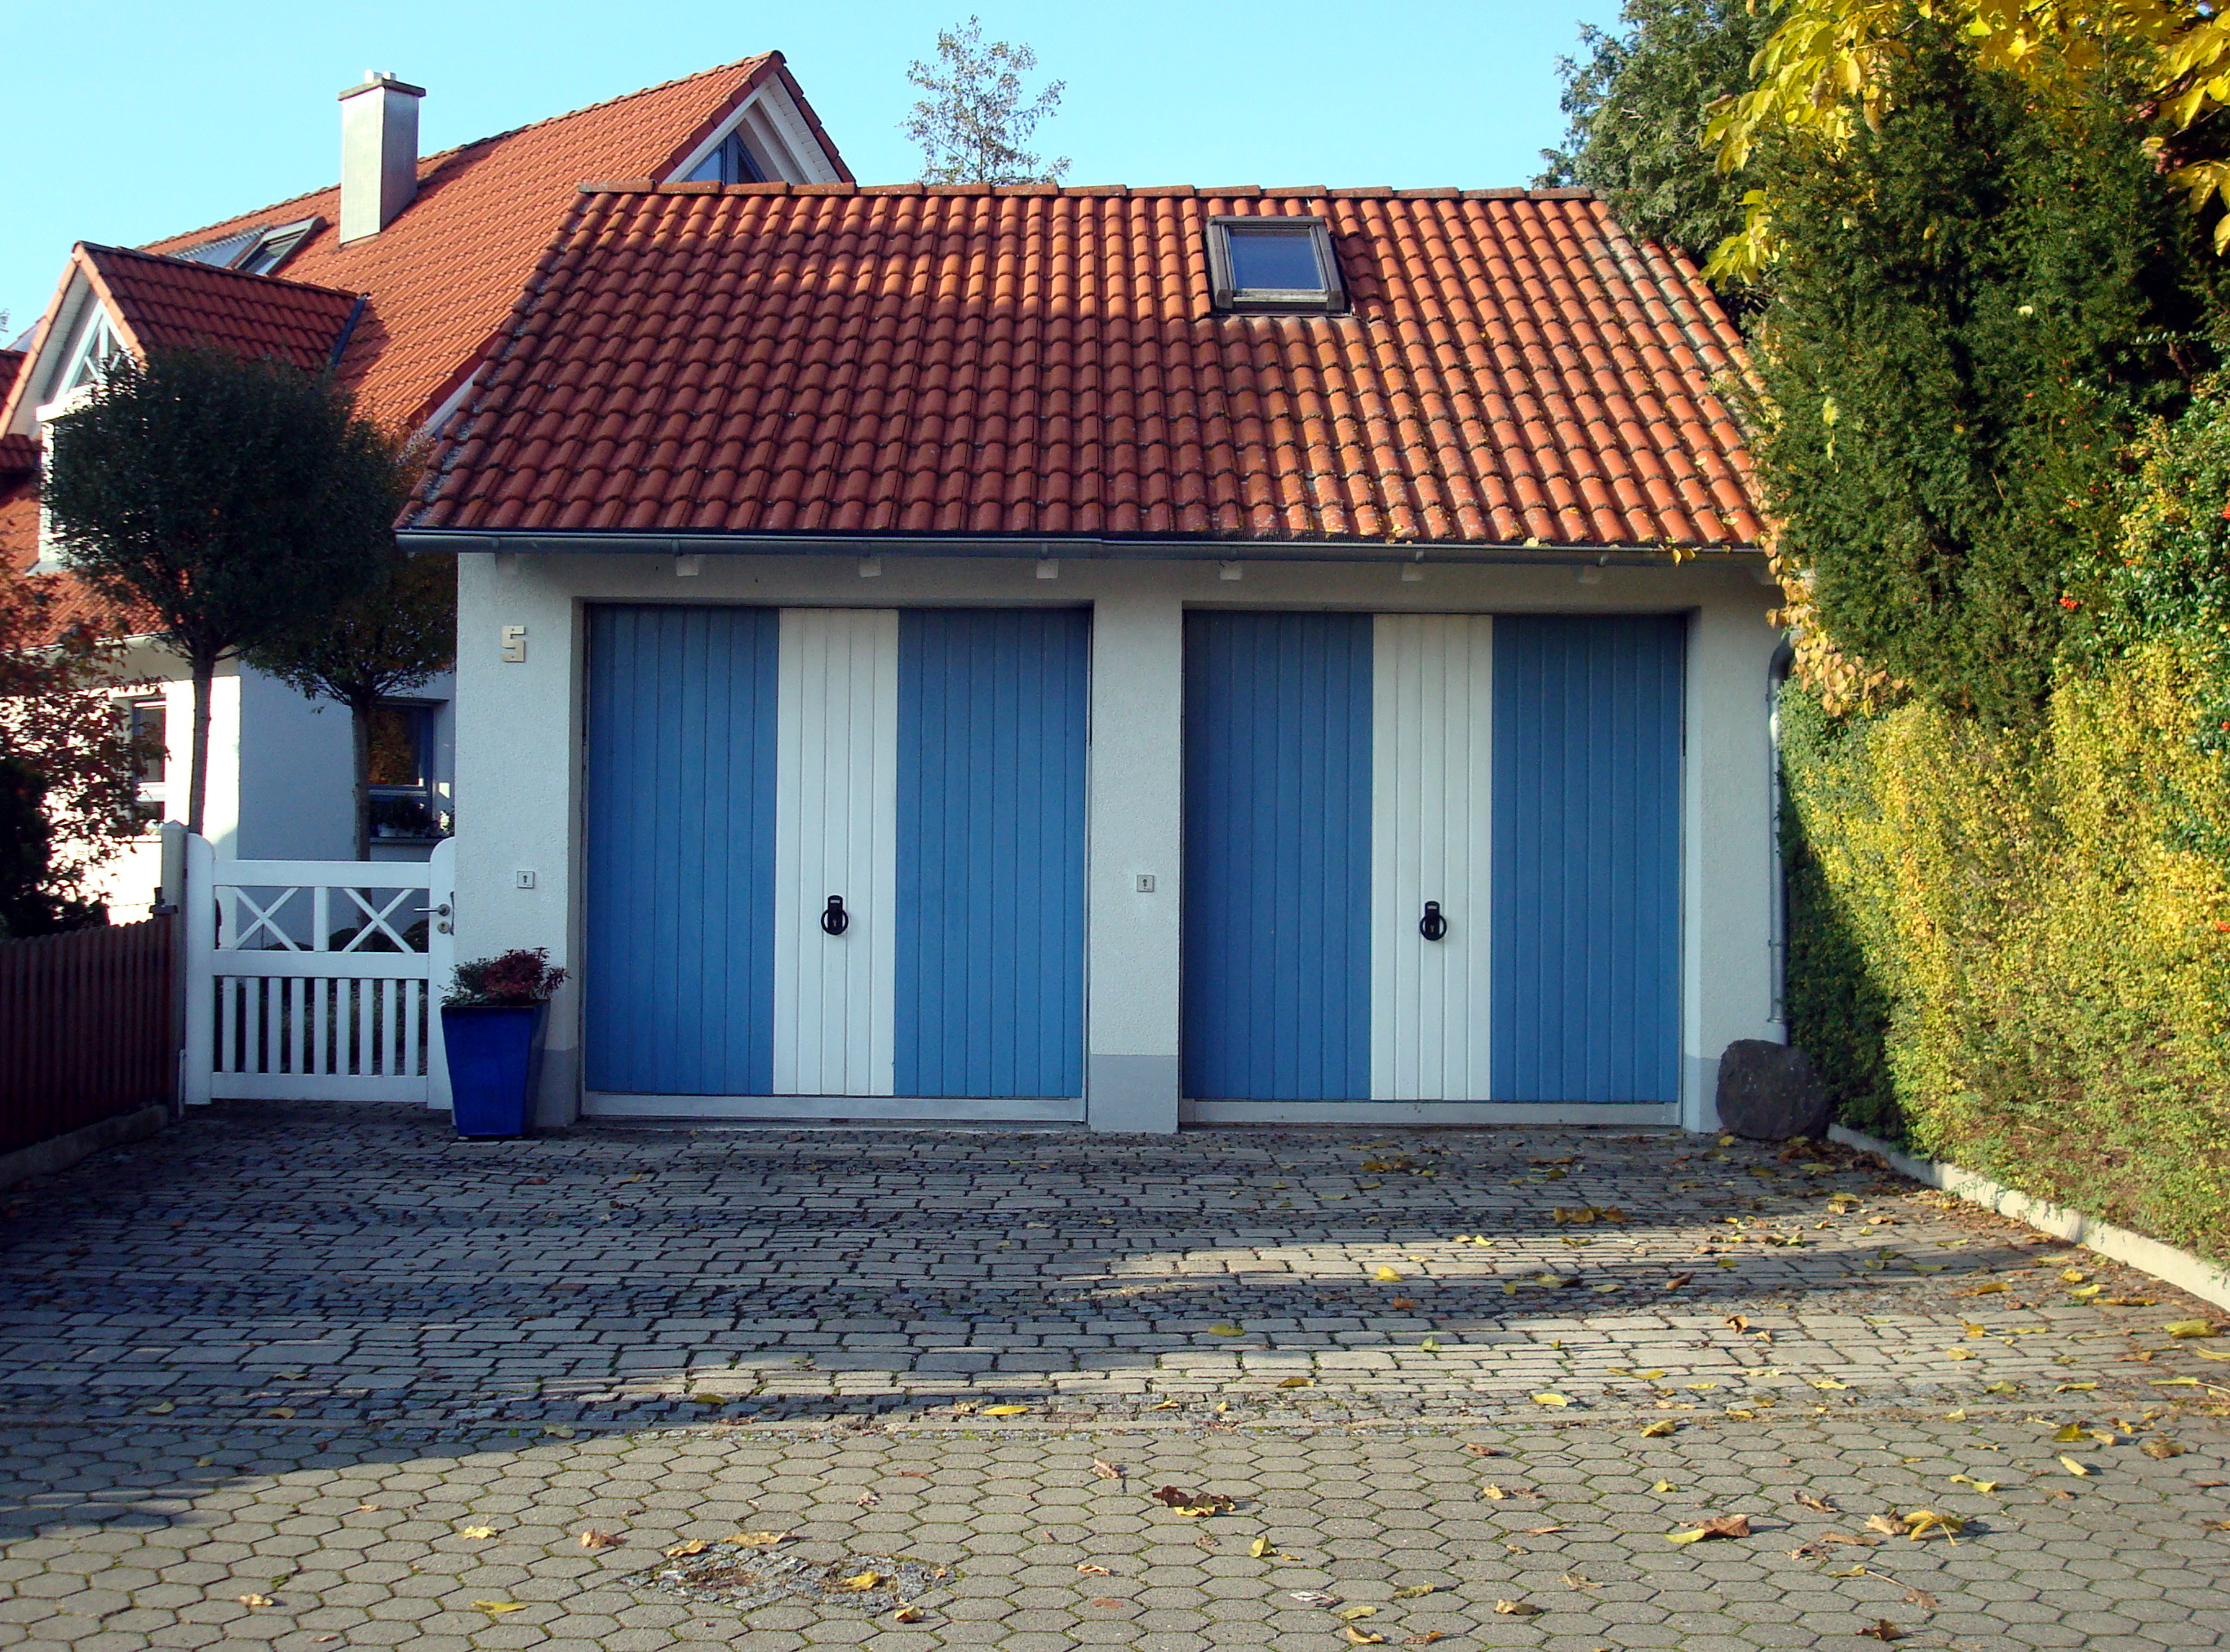
\includegraphics[width=0.9\textwidth]{Garage-Zu.jpg}}
\end{figure}
\end{frame}

%Rechte Garage offen
\begin{frame}{Problem}
\begin{figure}[h]
\makebox[\textwidth]{
 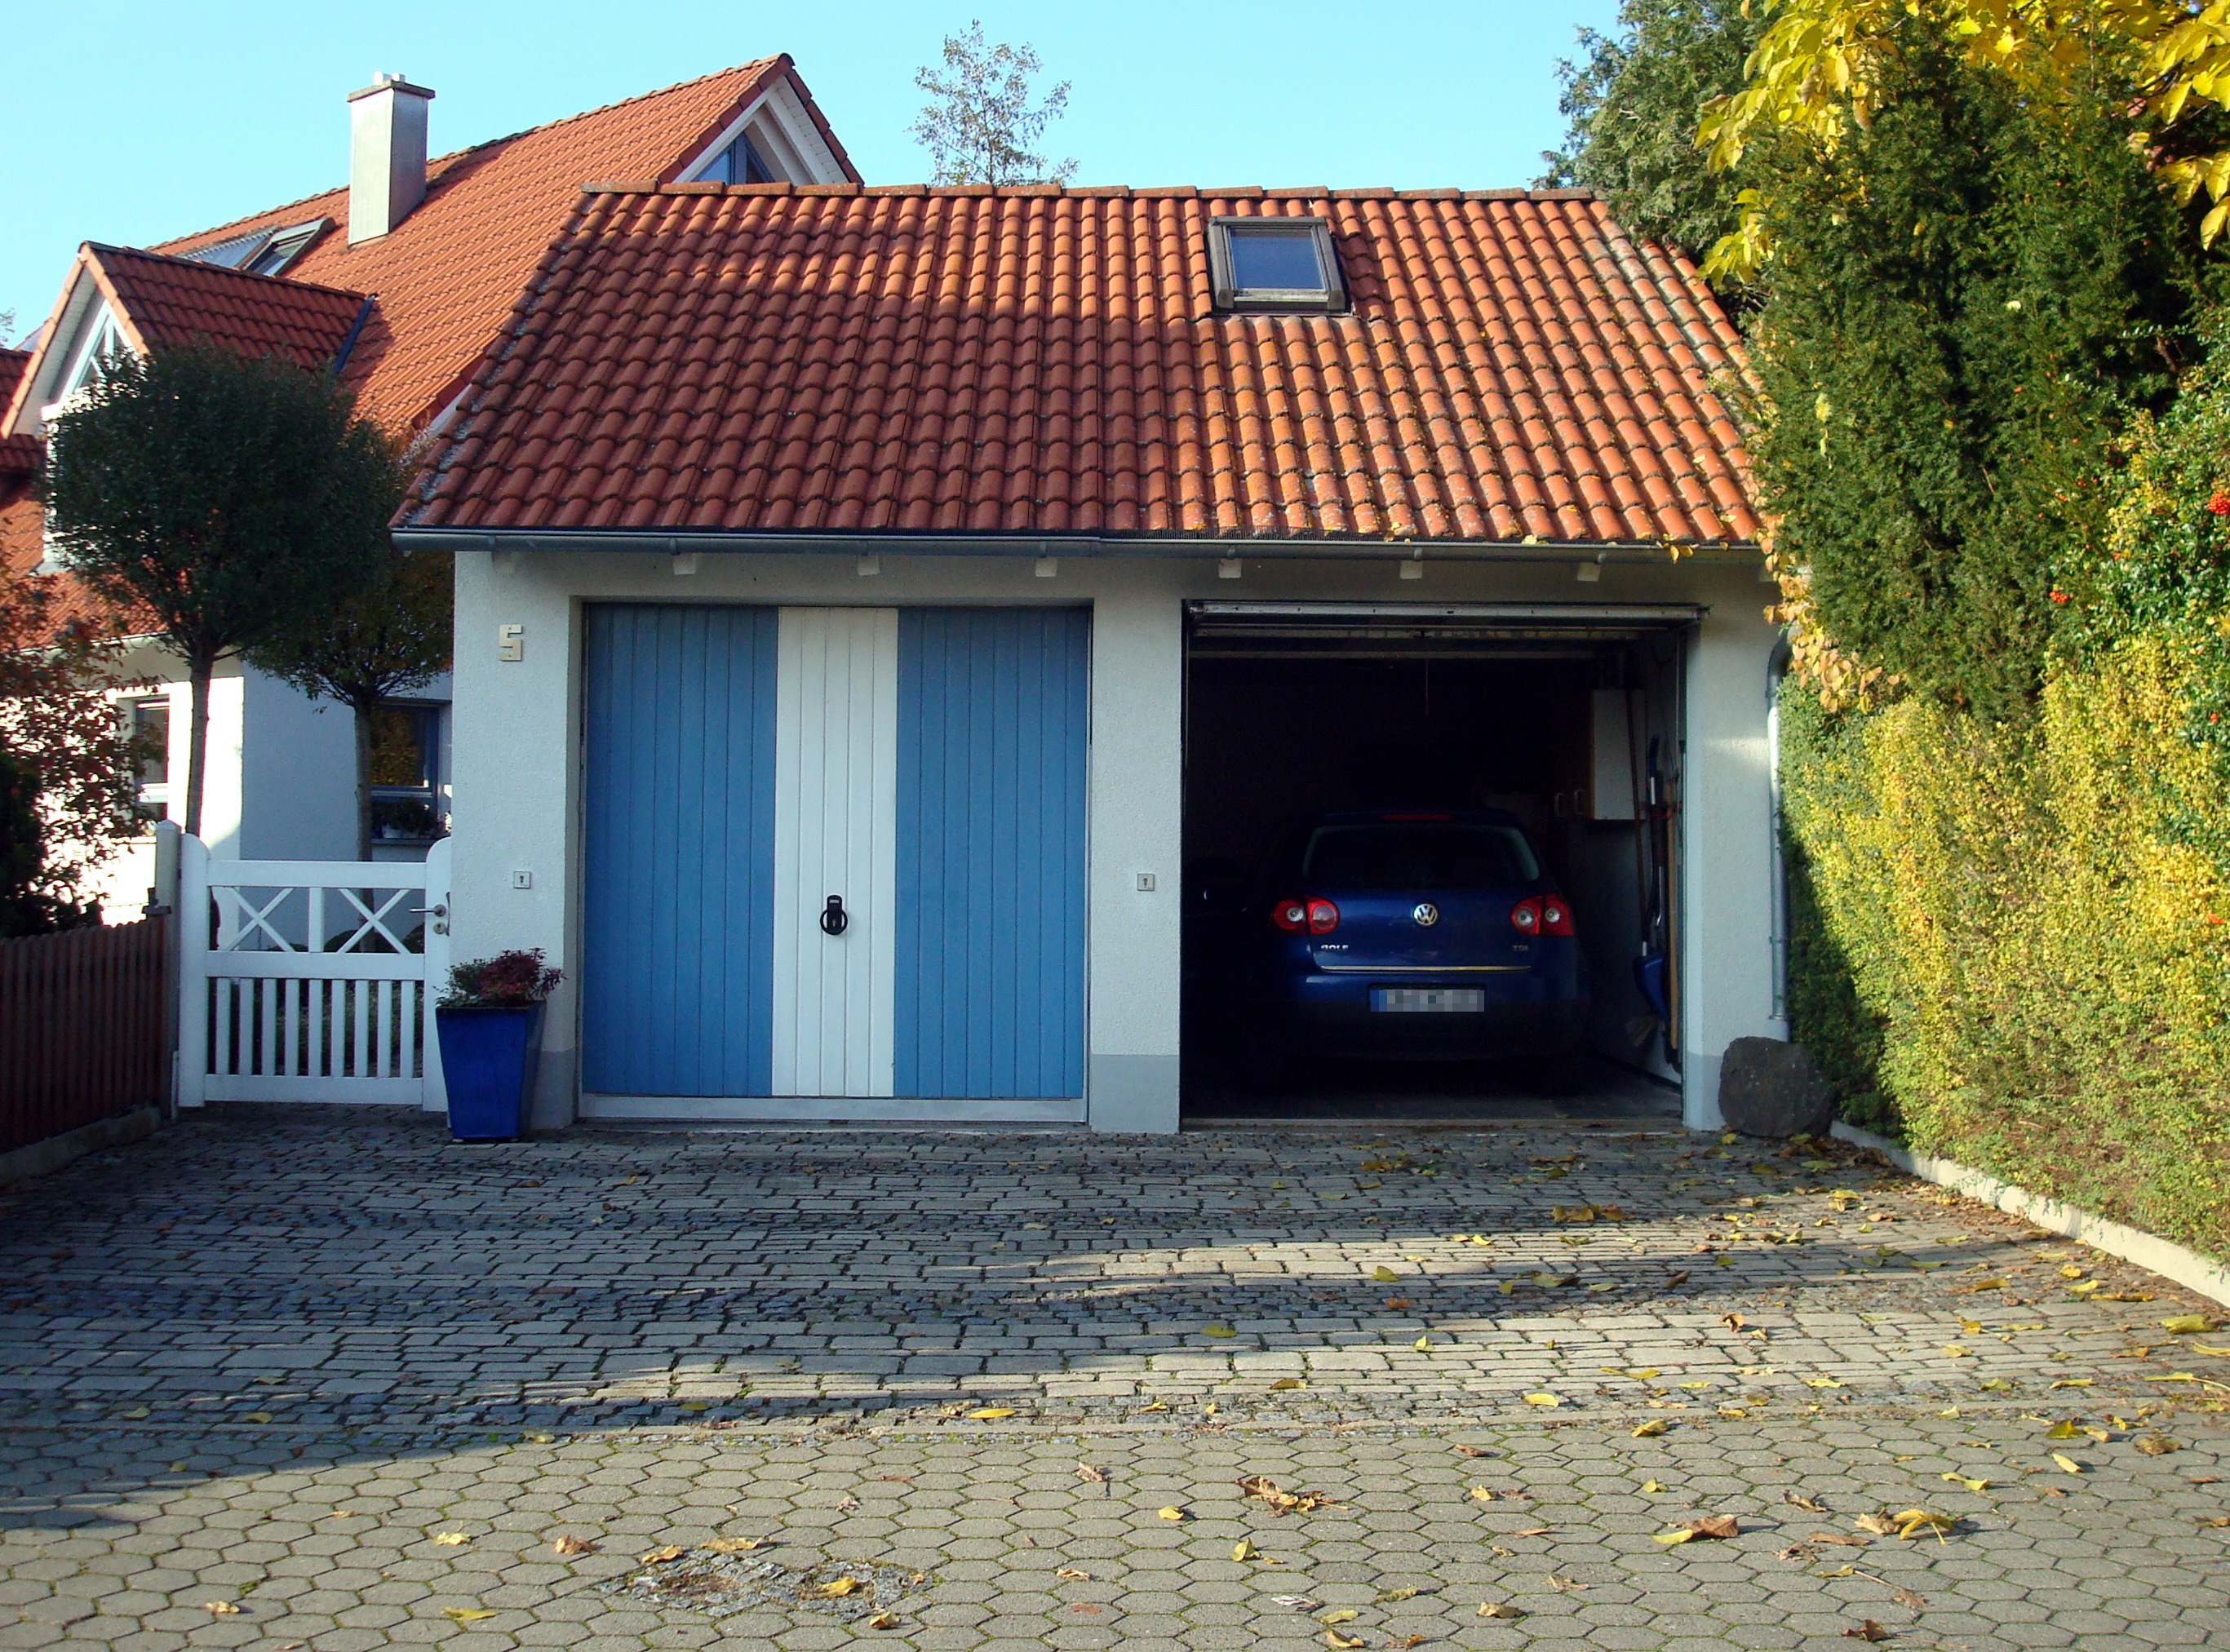
\includegraphics[width=0.9\textwidth]{Garage-Eins.jpg}}
\end{figure}
\end{frame}

%Beide Garagen offen
\begin{frame}{Problem}
\begin{figure}[h]
\makebox[\textwidth]{
 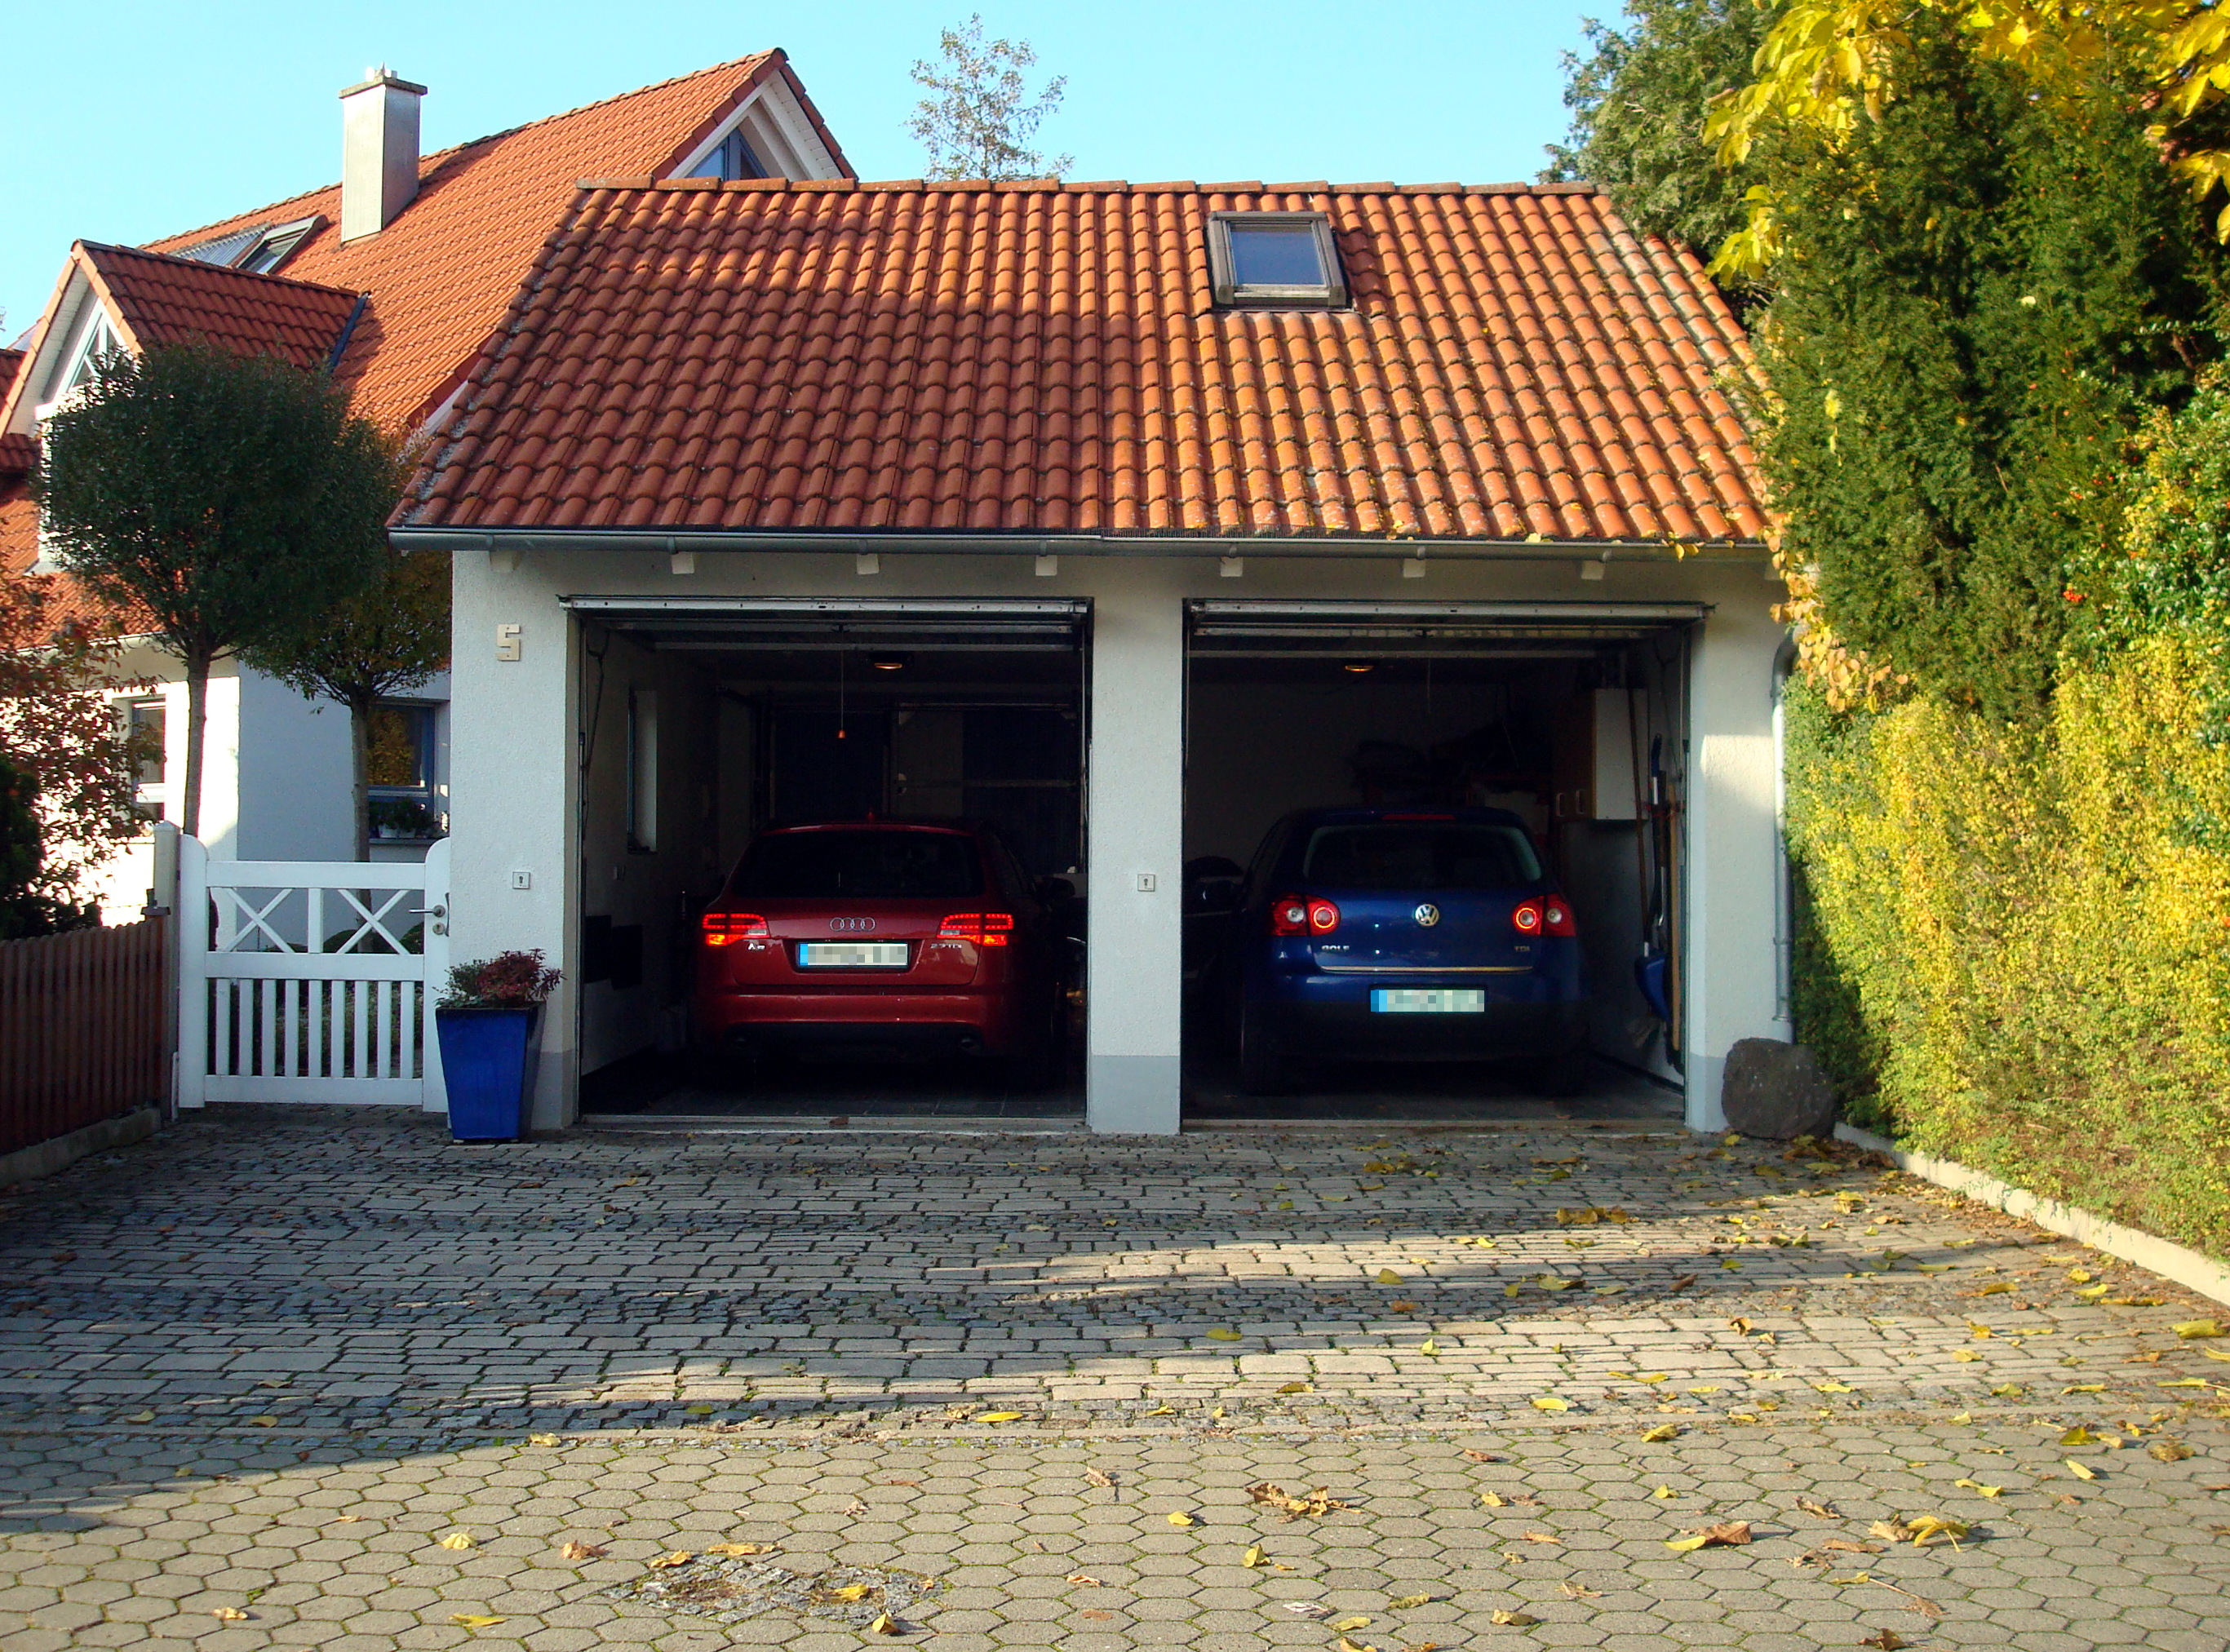
\includegraphics[width=0.9\textwidth]{Garage-Beide.jpg}}
\end{figure}
\end{frame}

%Garagen zu
\begin{frame}{Problem}
\begin{figure}[h]
\makebox[\textwidth]{
 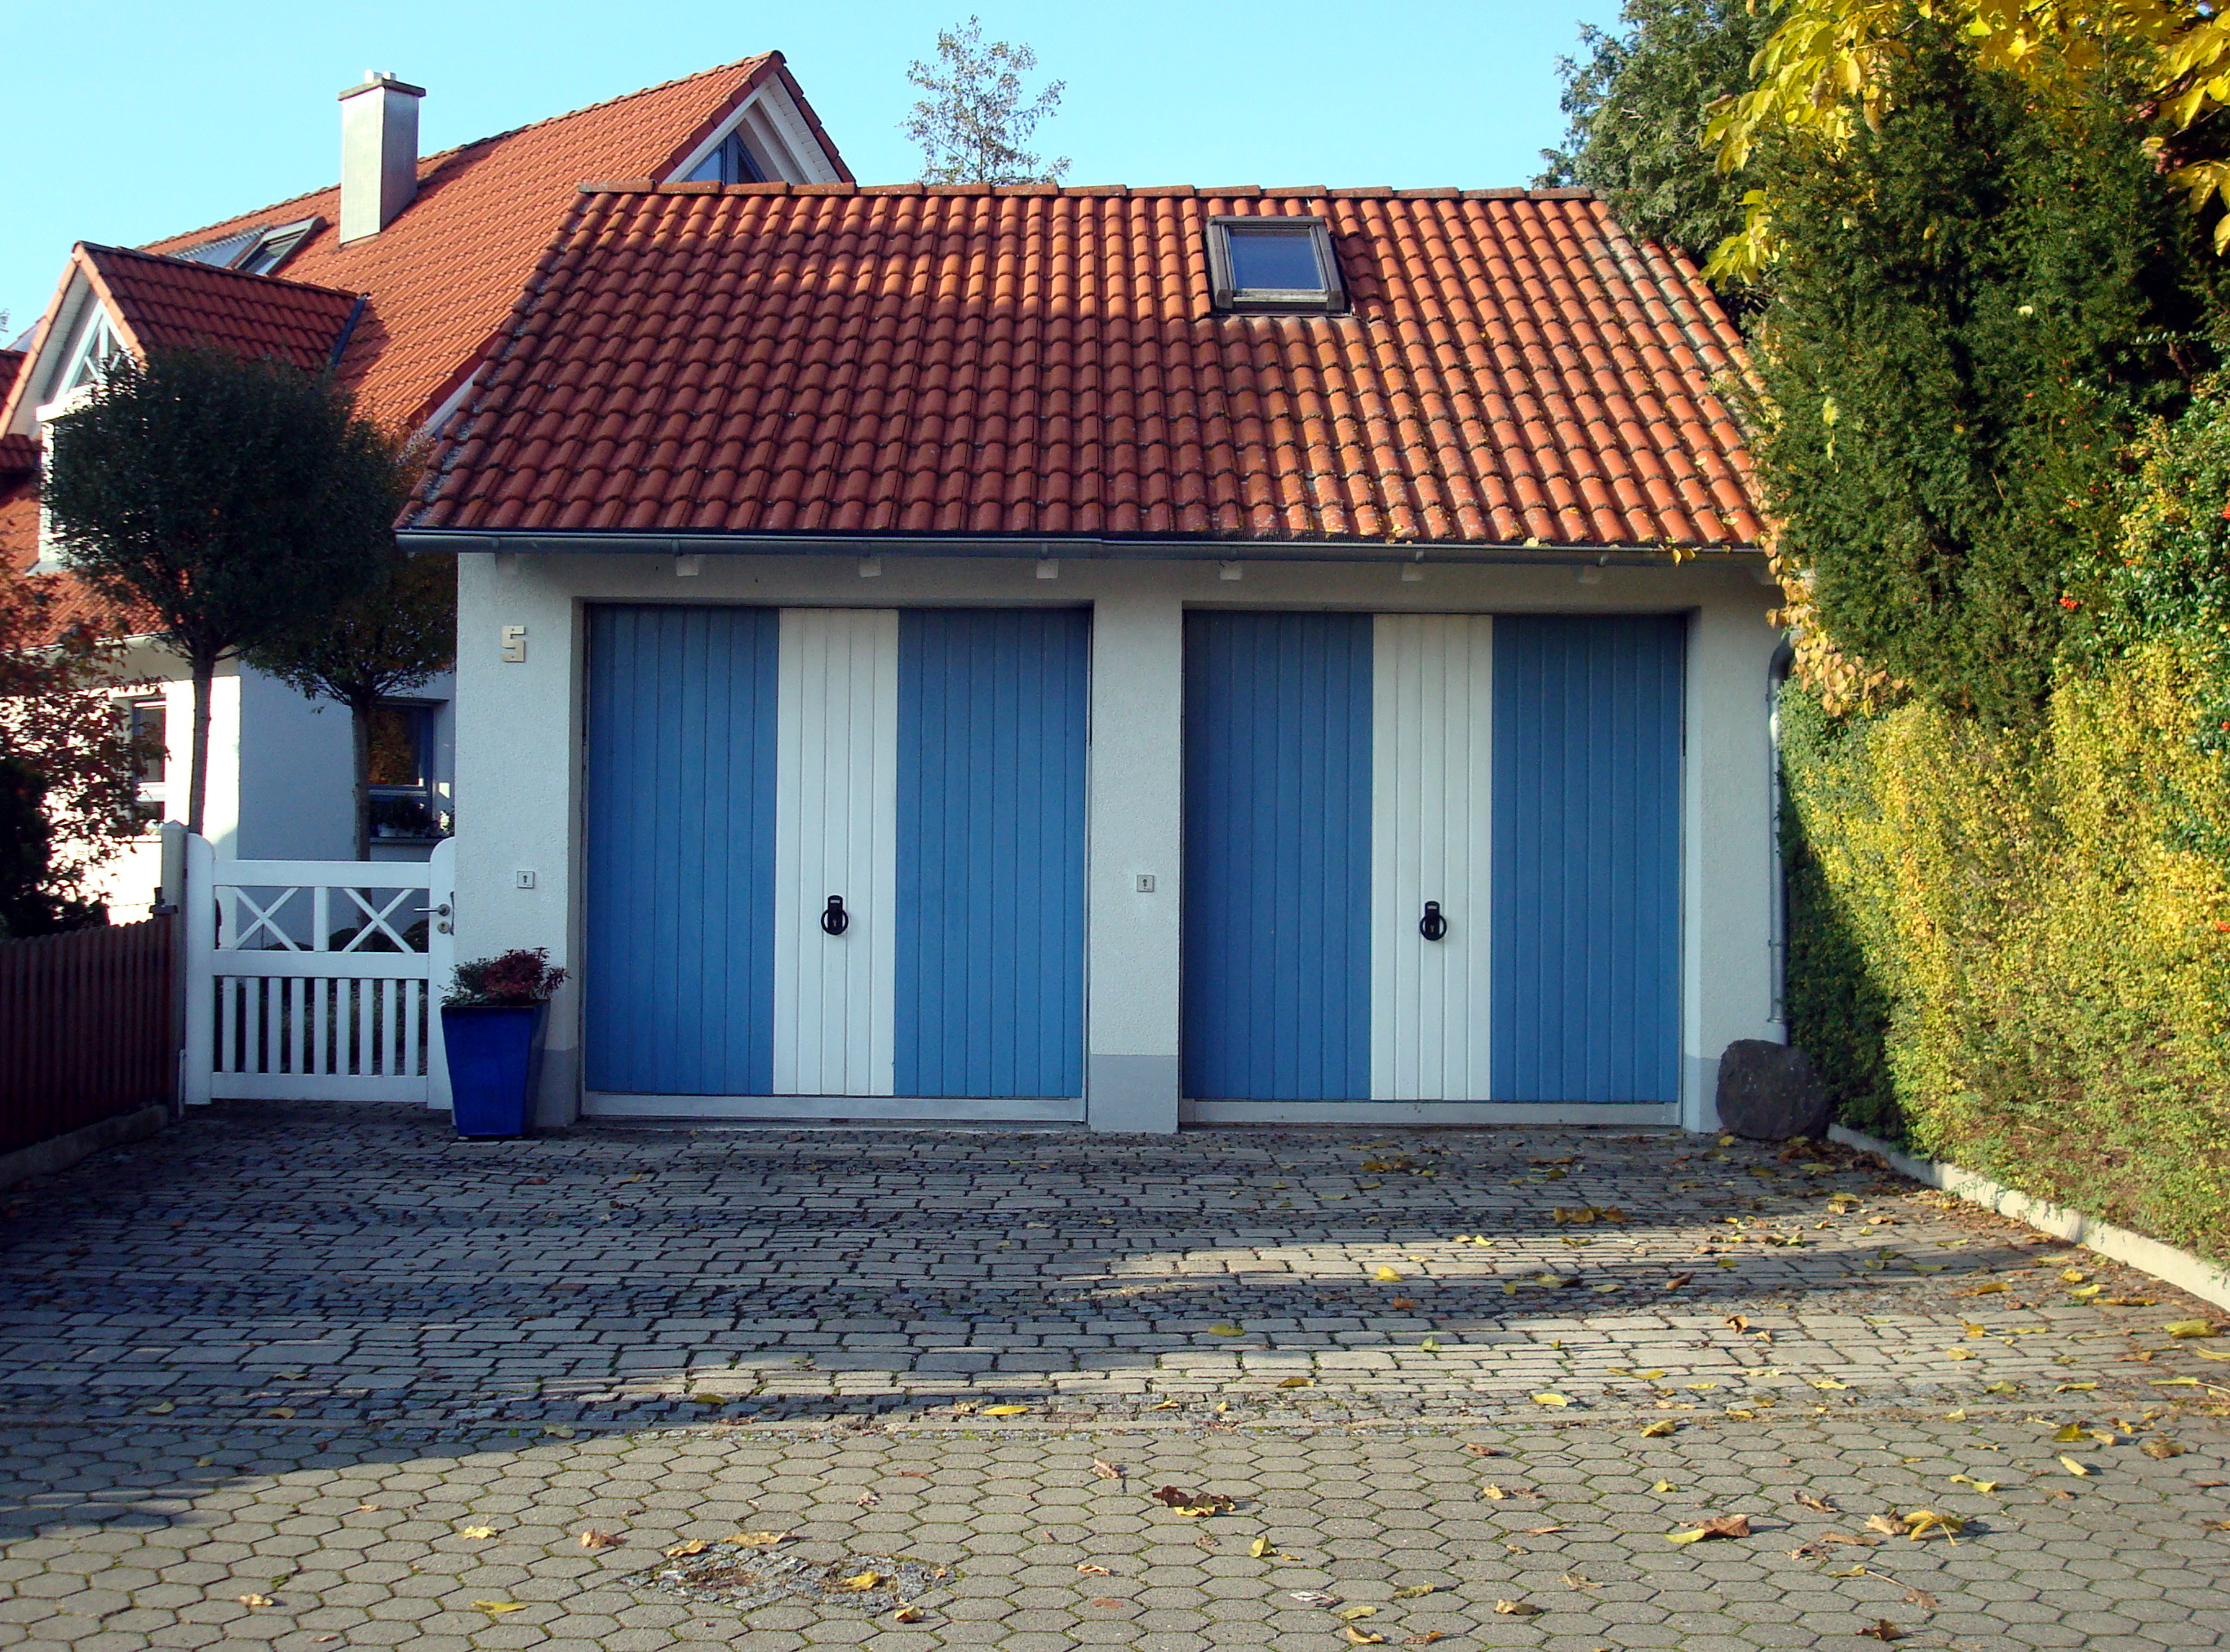
\includegraphics[width=0.9\textwidth]{Garage-Zu.jpg}}
\end{figure}
\end{frame}

%X-Ray!!!
\begin{frame}{Problem}
\begin{figure}[h]
\makebox[\textwidth]{
 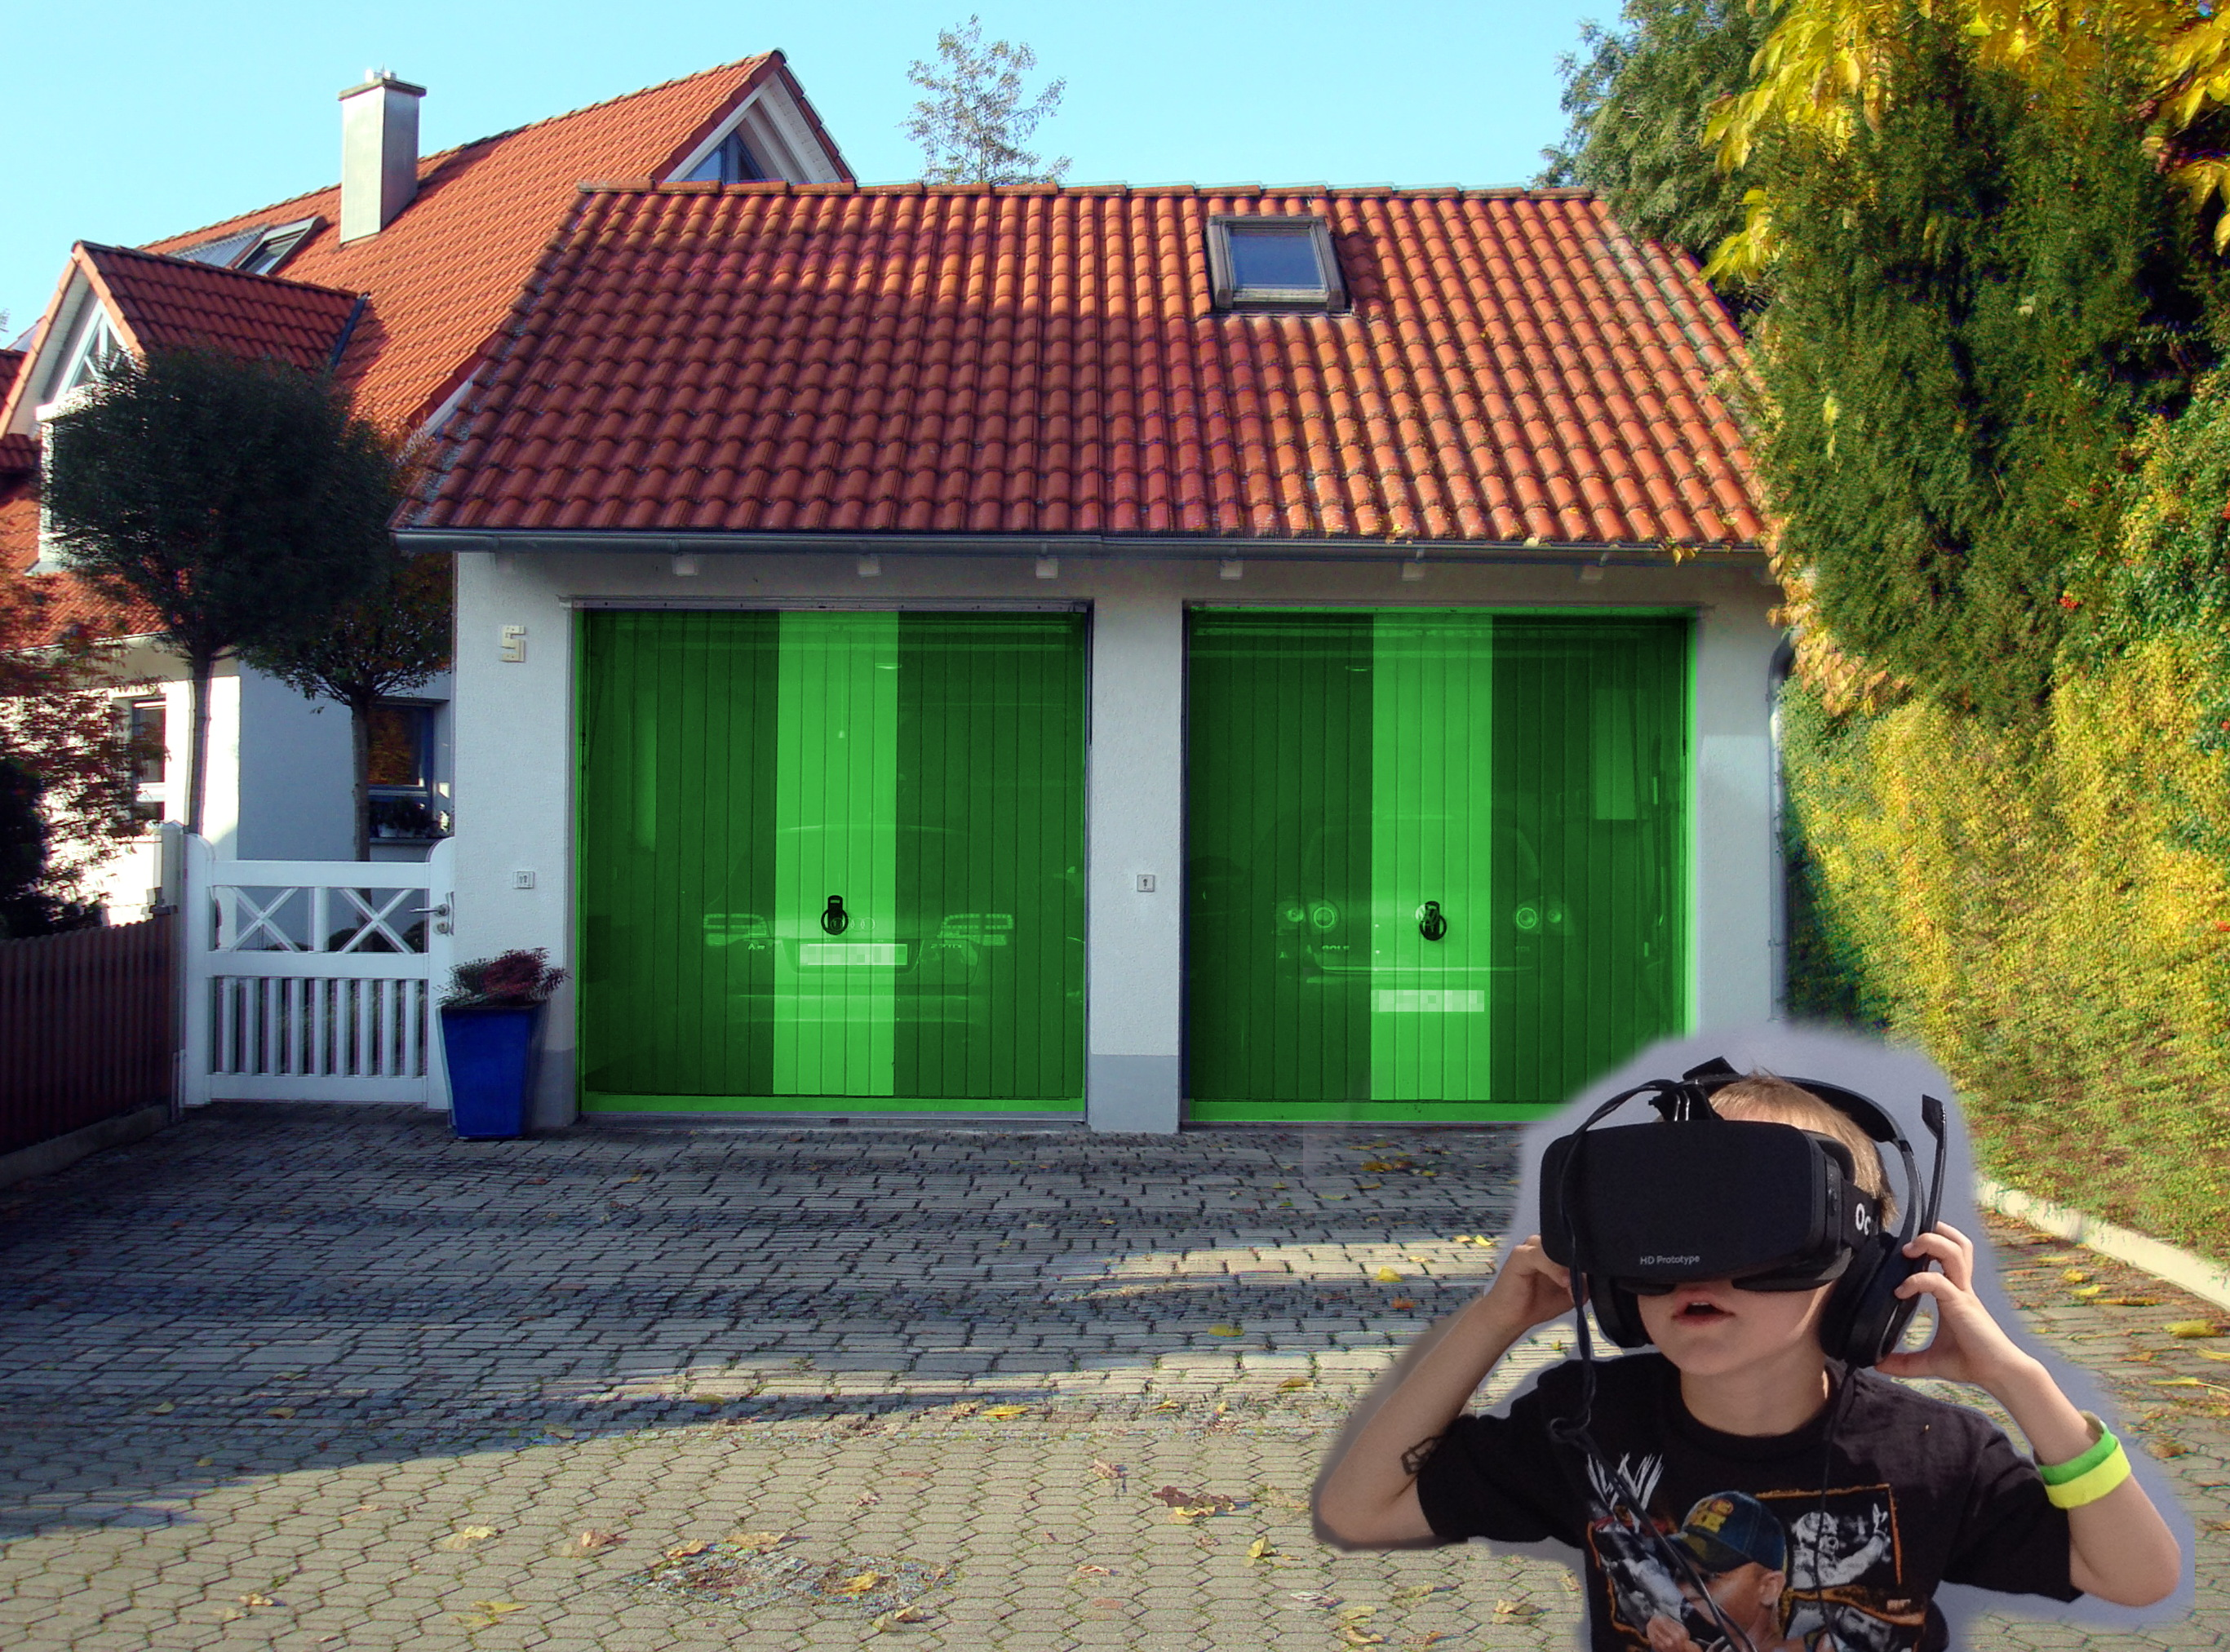
\includegraphics[width=0.9\textwidth]{Garage-X-Ray-2.jpg}}
\end{figure}
\end{frame}

%Garage geschlossen, mit Ampel
\begin{frame}{Lösung}
\begin{figure}[h]
\makebox[\textwidth]{
 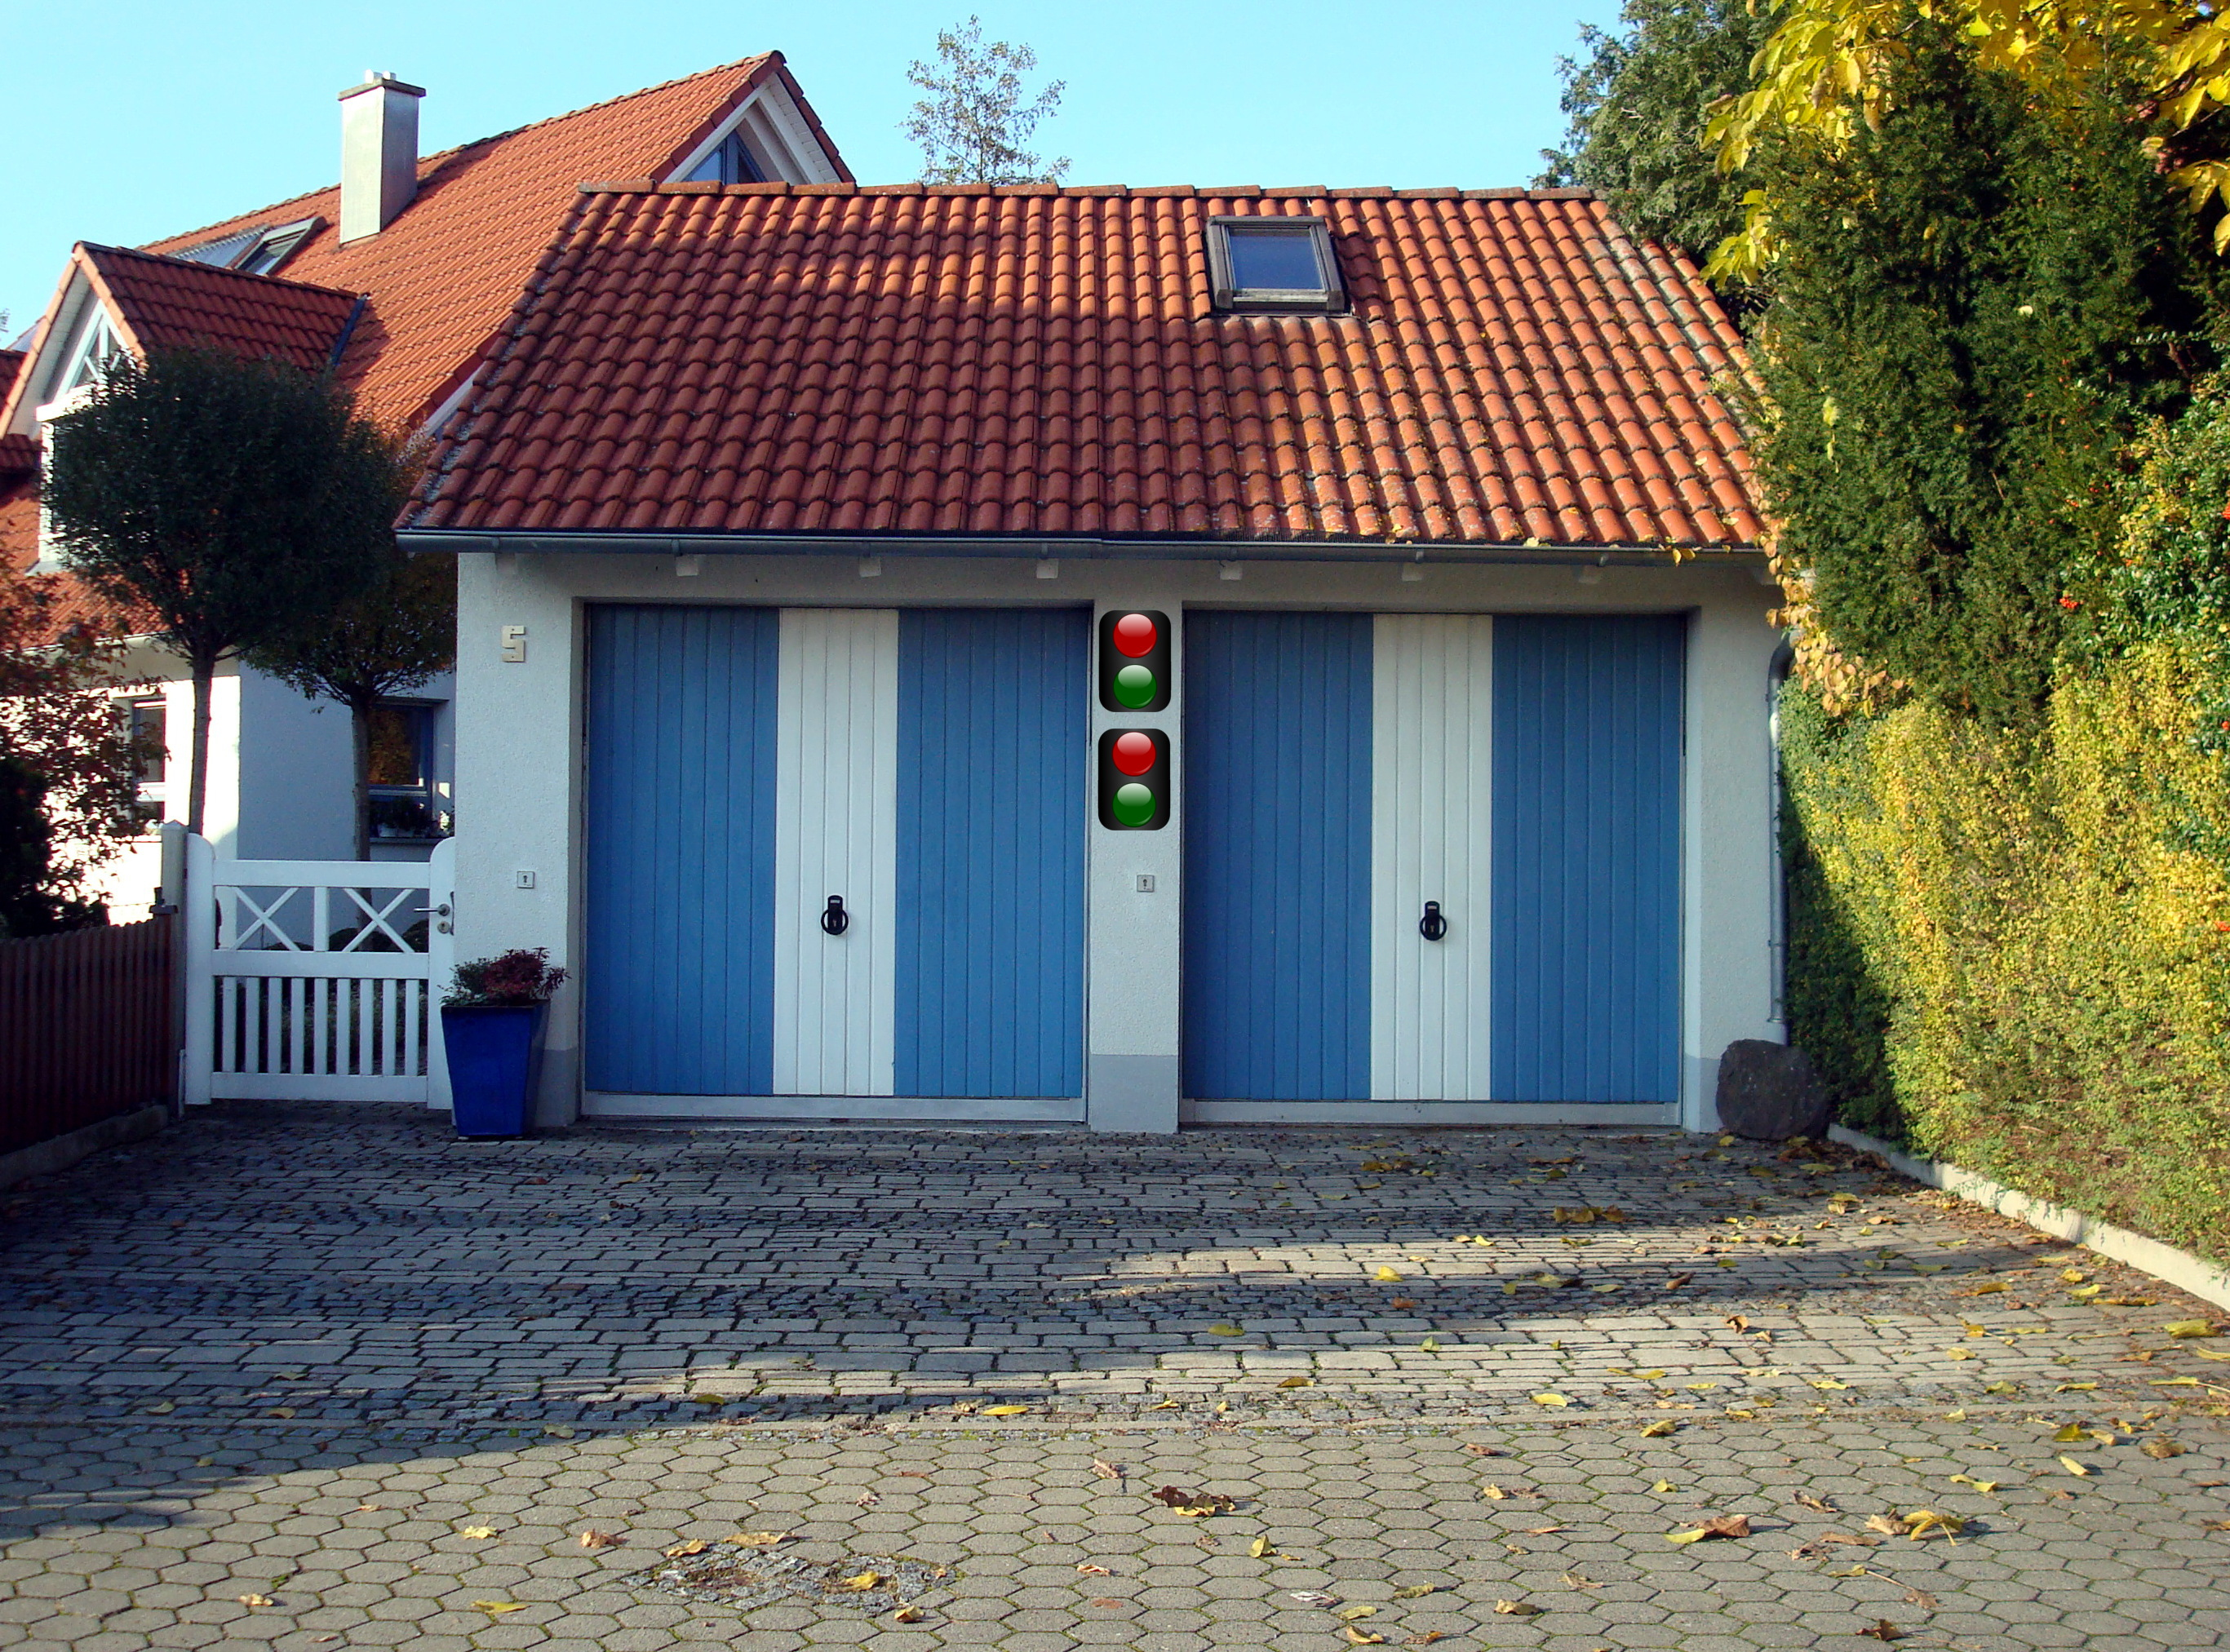
\includegraphics[width=0.9\textwidth]{Garage-Ampeln.jpg}}
\end{figure}
\end{frame}

%Garage geschlossen, mit Ampel durchgestrichen
\begin{frame}{ ... doch nicht}
\begin{figure}[h]
\makebox[\textwidth]{
 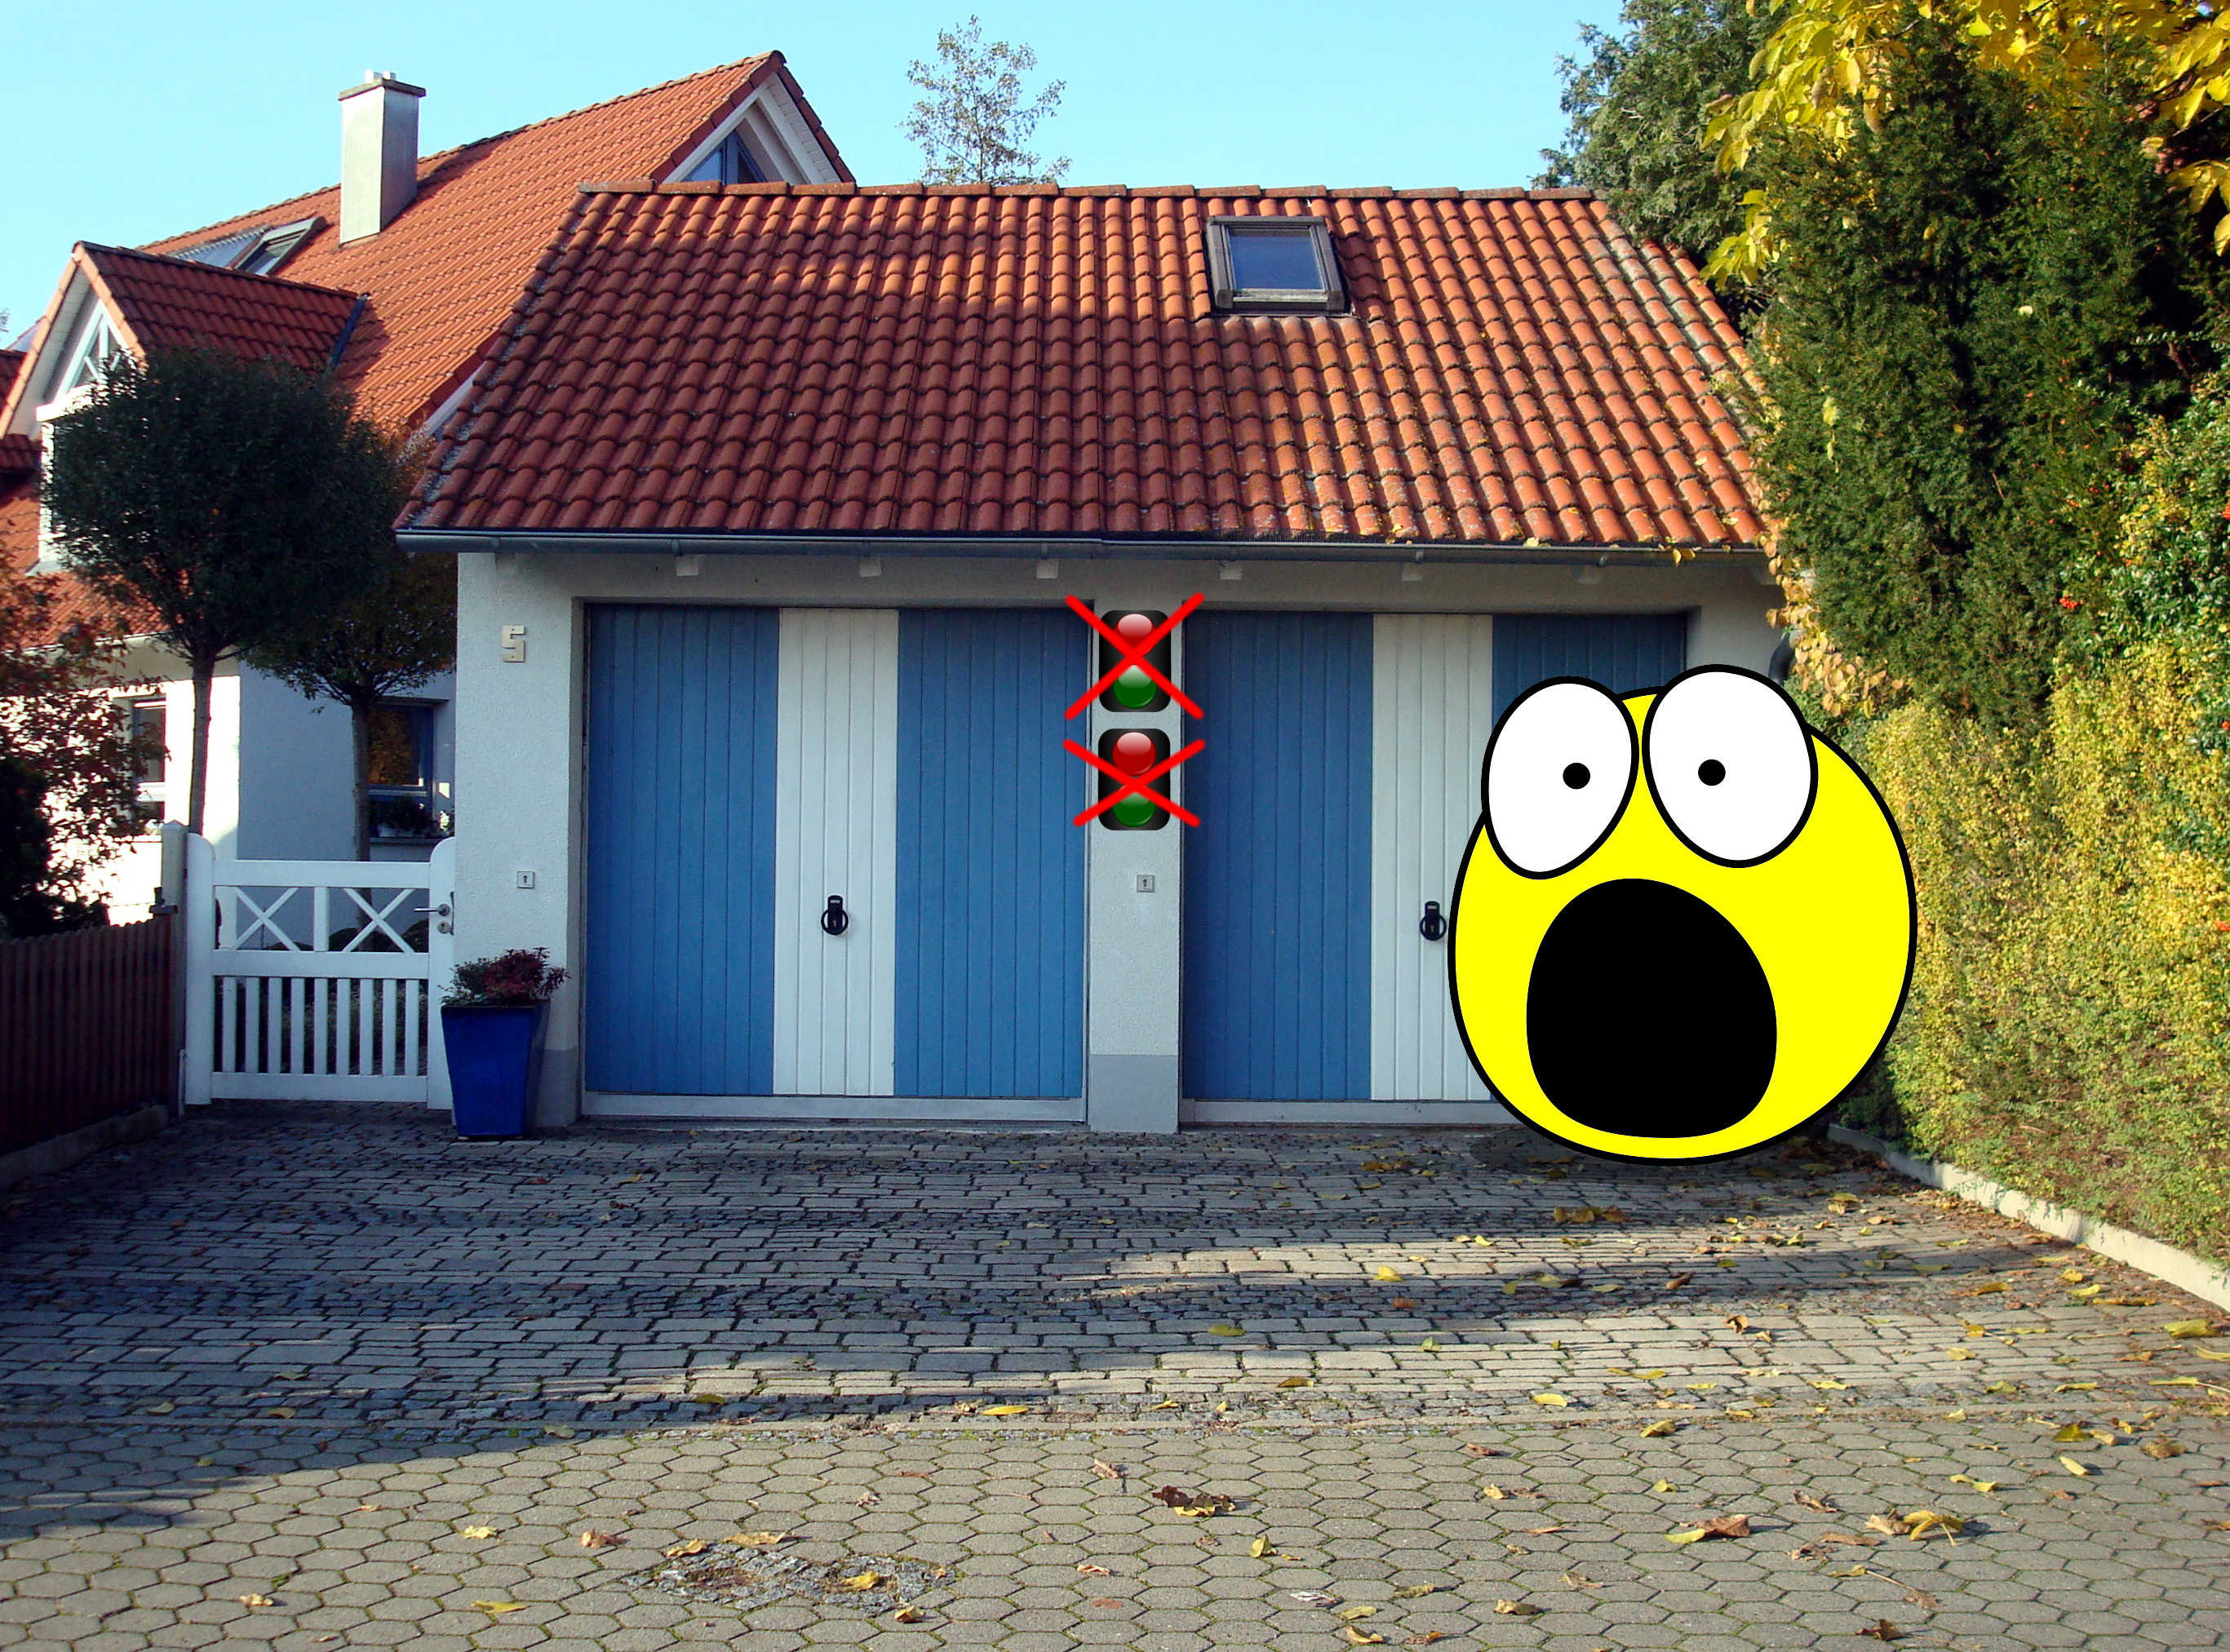
\includegraphics[width=0.9\textwidth]{Garage-Ampeln-Smiley-durchgestrichen.jpg}}
\end{figure}
\end{frame}

%Lösung
\begin{frame}{Lösung}
\begin{figure}[h]
\makebox[\textwidth]{
 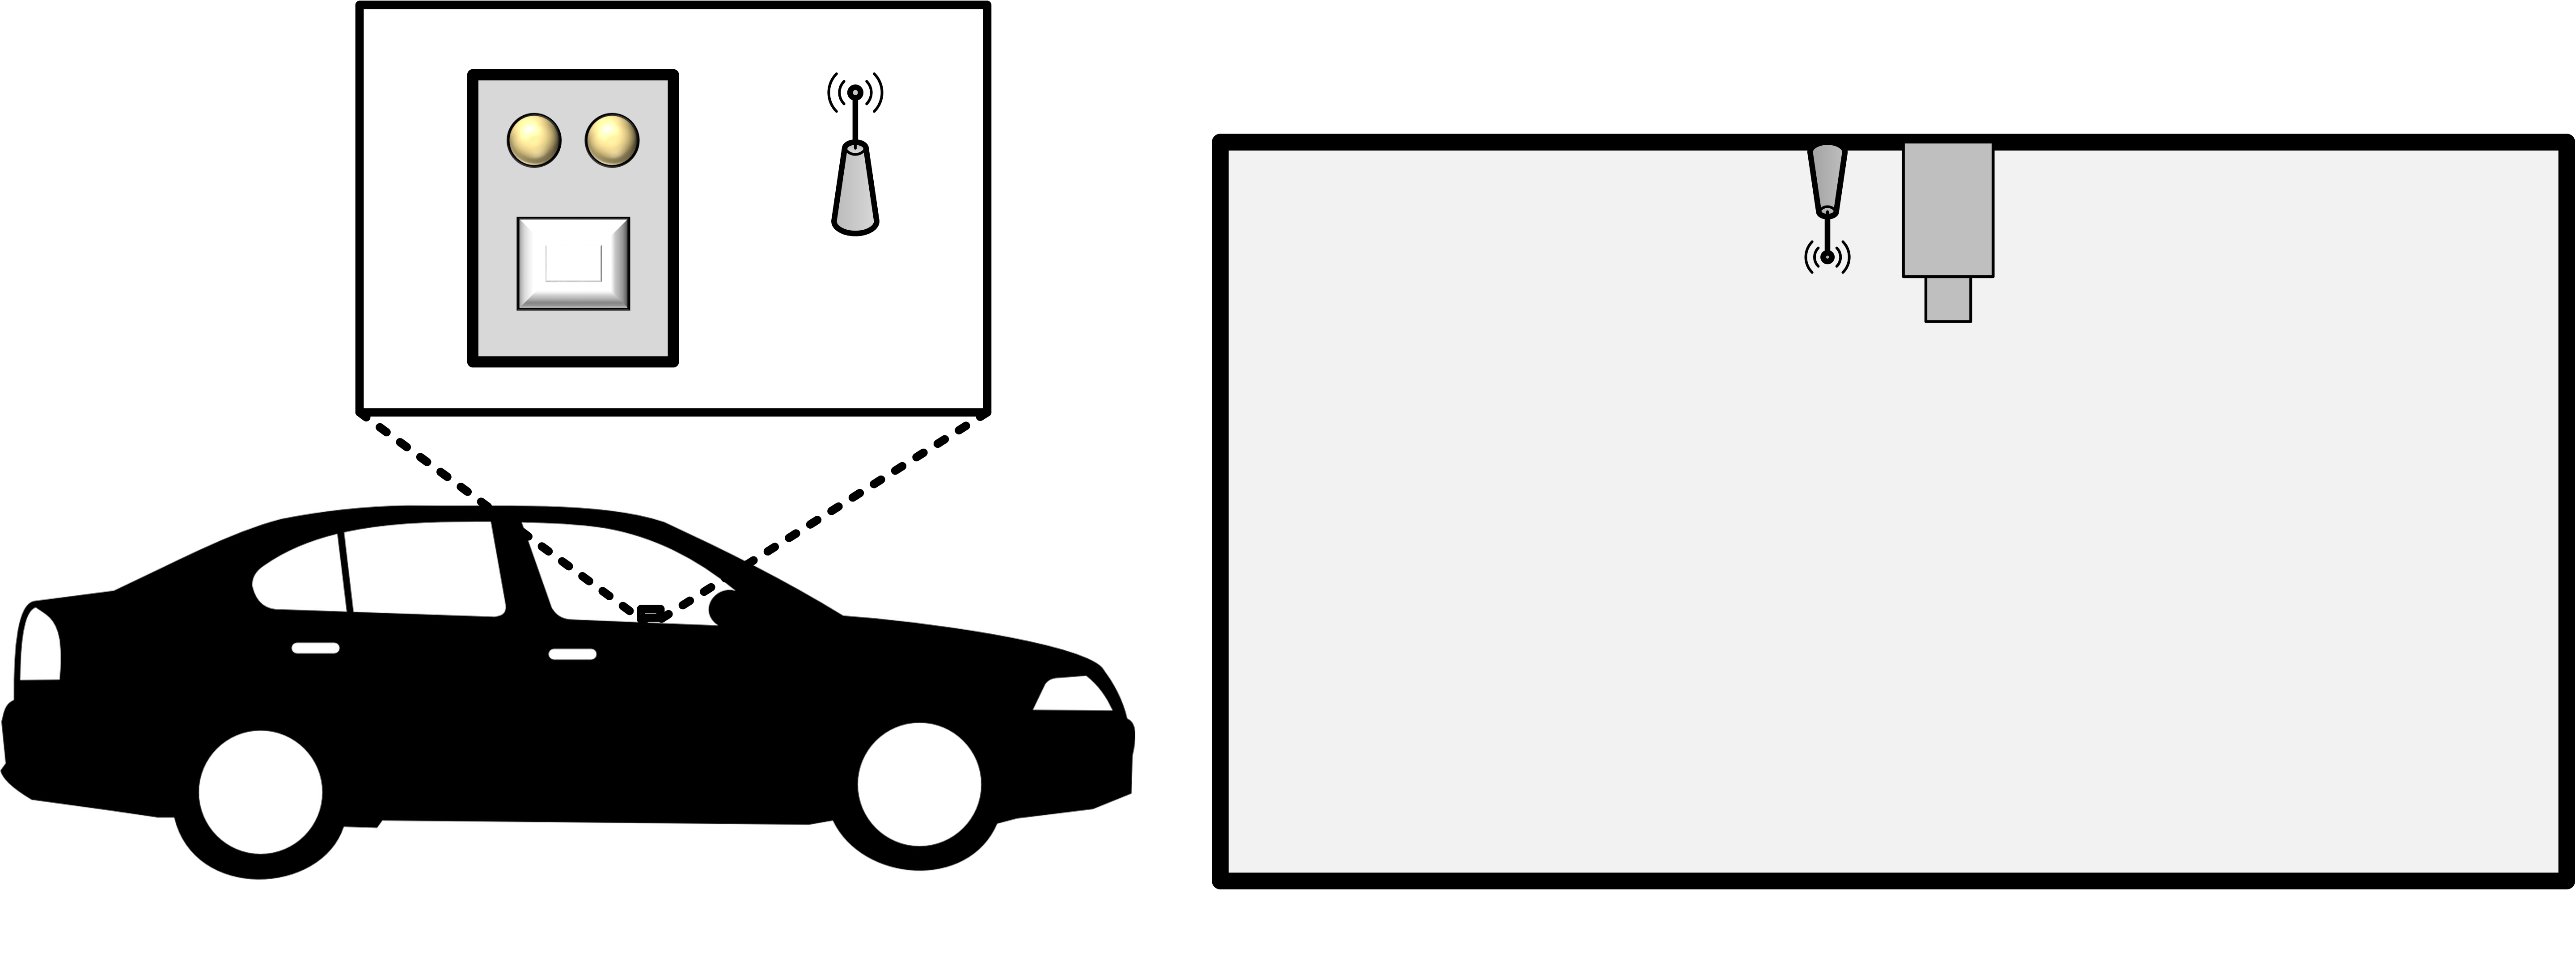
\includegraphics[width=1.0\textwidth]{Garagenzeichnung-Sensor-ohne-Strahl.png}}
\end{figure}
\end{frame}

%Lösung
\begin{frame}{Lösung}
\begin{figure}[h]
\makebox[\textwidth]{
 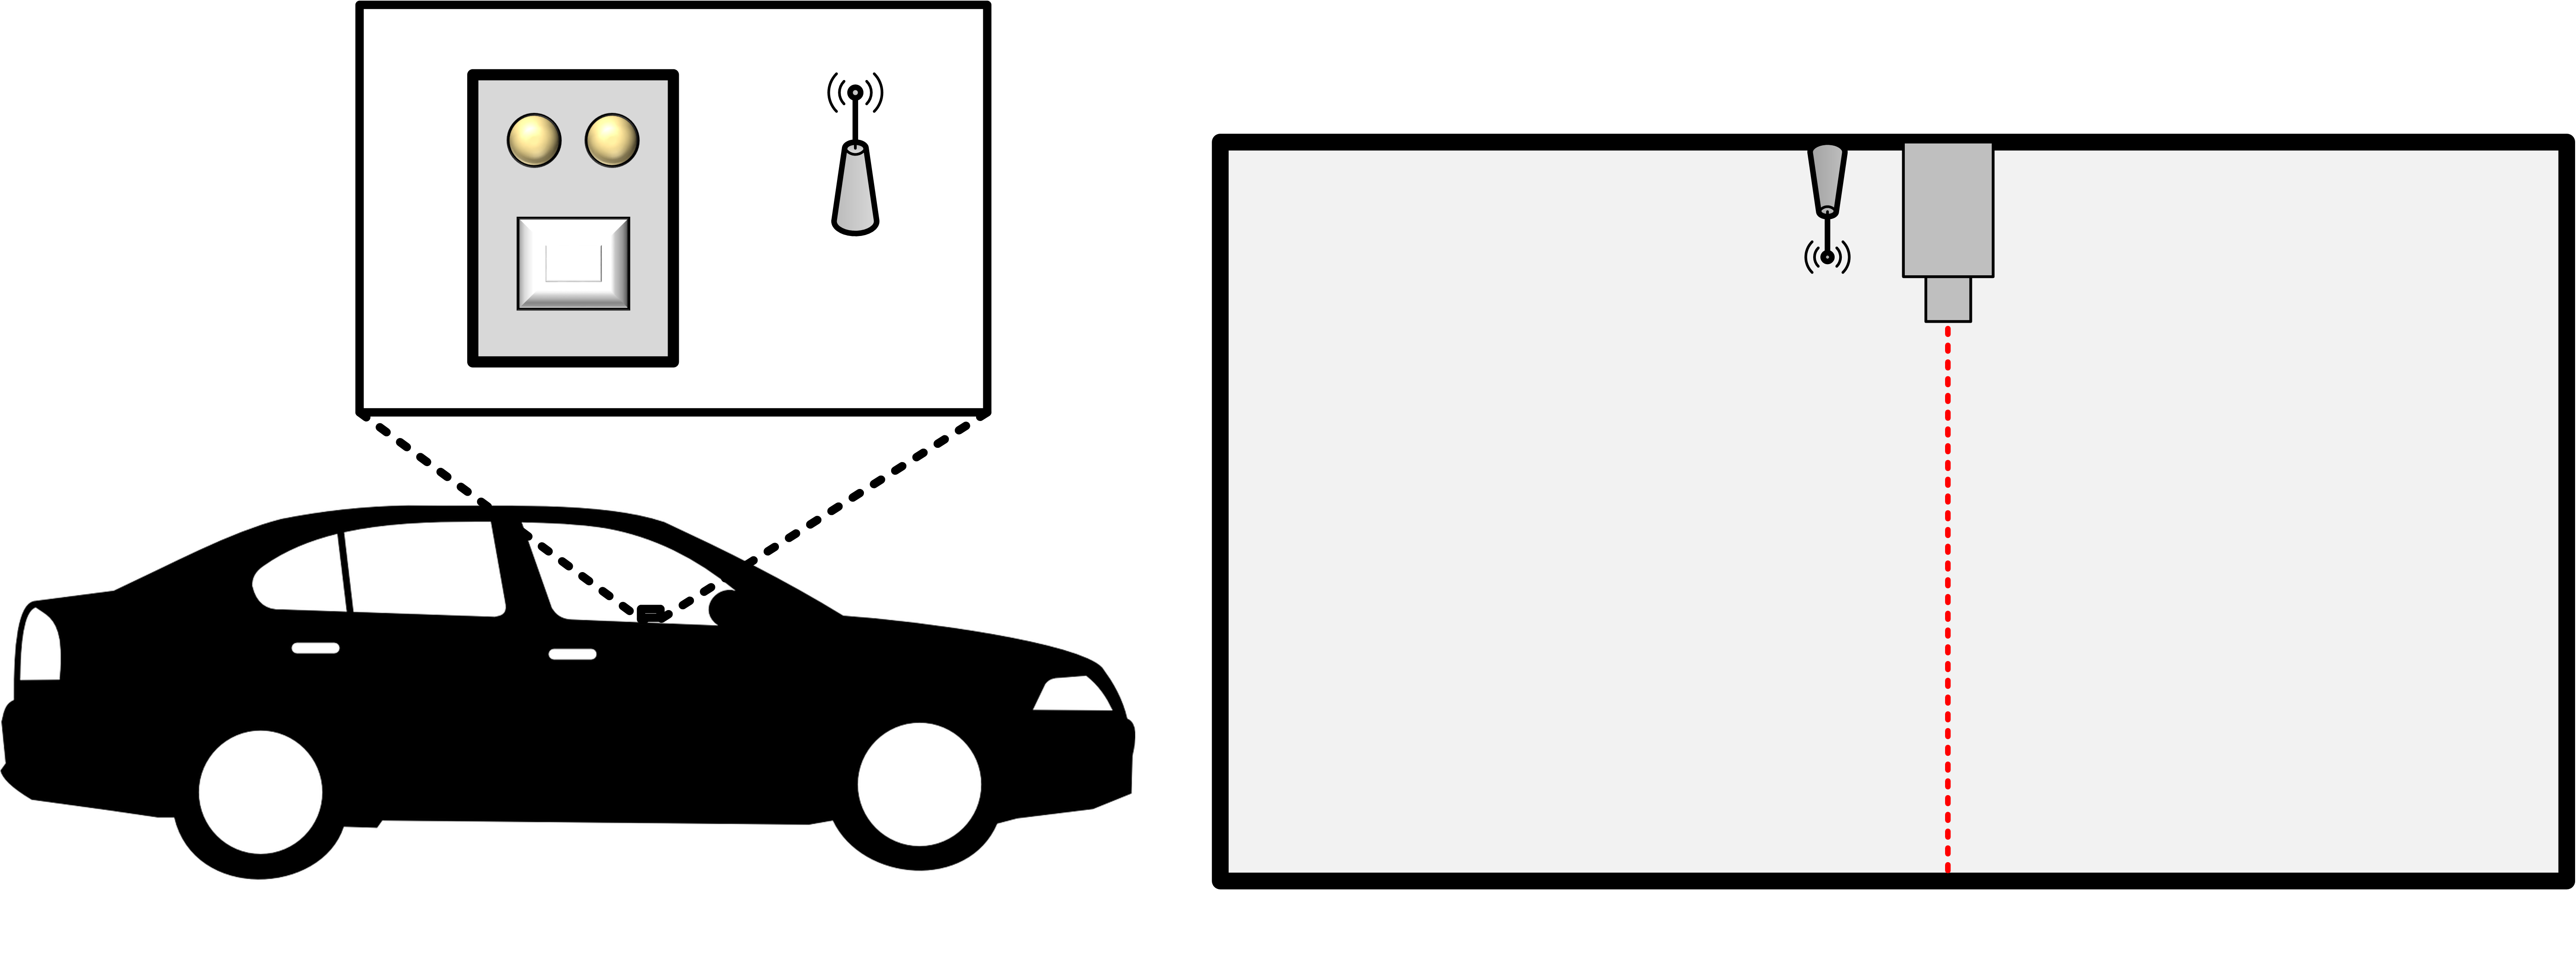
\includegraphics[width=1.0\textwidth]{Garagenzeichnung-Sensor-leer.png}}
\end{figure}
\end{frame}

%Lösung
\begin{frame}{Lösung}
\begin{figure}[h]
\makebox[\textwidth]{
 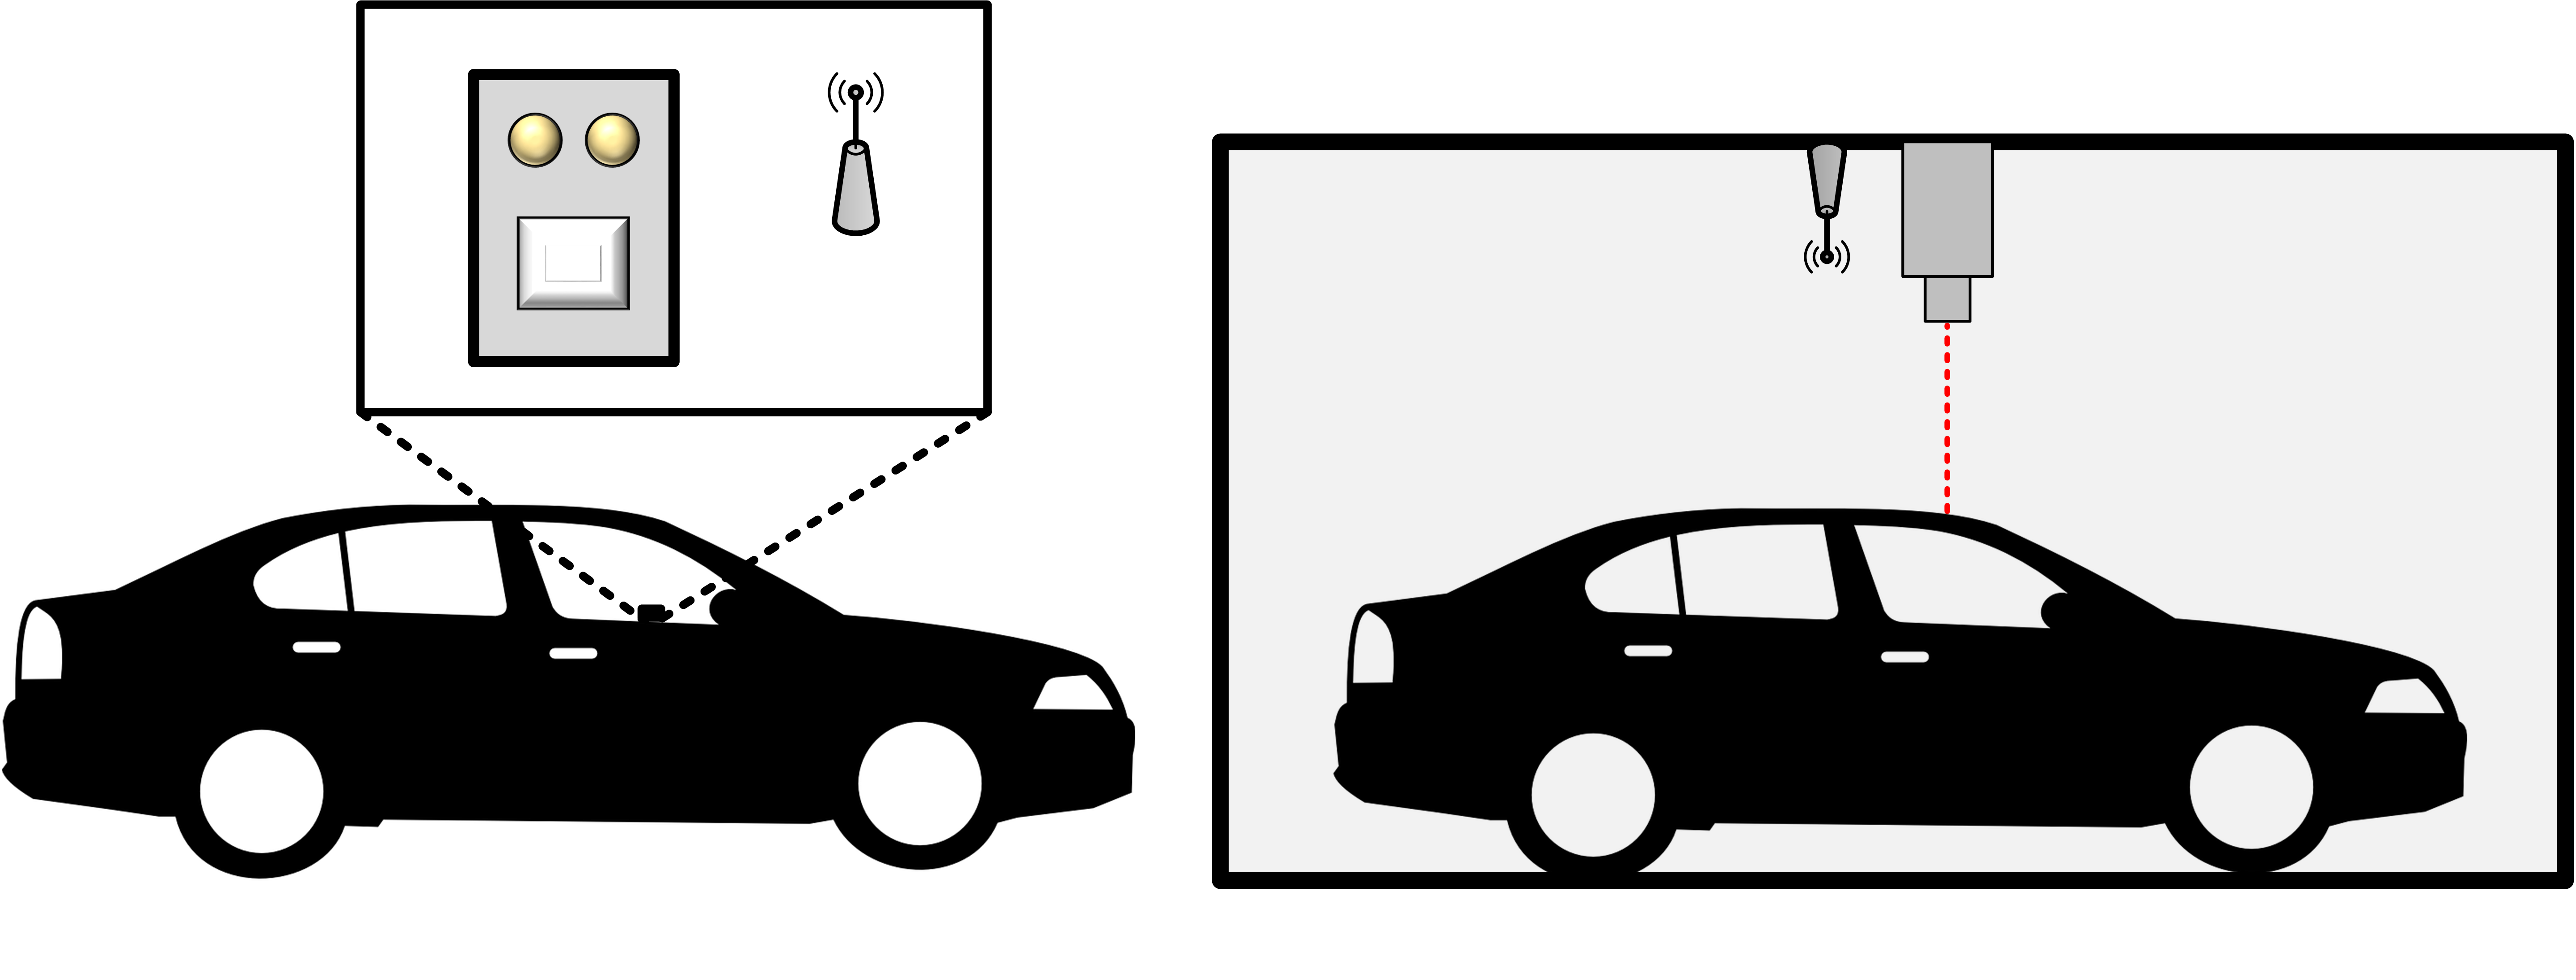
\includegraphics[width=1.0\textwidth]{Garagenzeichnung-Sensor-mit-Auto.png}}
\end{figure}
\end{frame}

\end{document}